%%
%% This is file `sigconf.tex',
%% generated with the docstrip utility.
%%
%% The original source files were:
%%
%% samples.dtx  (with options: `all,proceedings,sigconf')
%% 
%% IMPORTANT NOTICE:
%% 
%% For the copyright see the source file.
%% 
%% Any modified versions of this file must be renamed
%% with new filenames distinct from sigconf.tex.
%% 
%% For distribution of the original source see the terms
%% for copying and modification in the file samples.dtx.
%% 
%% This generated file may be distributed as long as the
%% original source files, as listed above, are part of the
%% same distribution. (The sources need not necessarily be
%% in the same archive or directory.)
%%
%%
%% Commands for TeXCount
%TC:macro \cite [option:text,text]
%TC:macro \citep [option:text,text]
%TC:macro \citet [option:text,text]
%TC:envir table 0 1
%TC:envir table* 0 1
%TC:envir tabular [ignore] word
%TC:envir displaymath 0 word
%TC:envir math 0 word
%TC:envir comment 0 0
%%
%% The first command in your LaTeX source must be the \documentclass
%% command.
%%
%% For submission and review of your manuscript please change the
%% command to \documentclass[manuscript, screen, review]{acmart}.
%%
%% When submitting camera ready or to TAPS, please change the command
%% to \documentclass[sigconf]{acmart} or whichever template is required
%% for your publication.
%%
%%
\documentclass[11pt,sigconf,nonacm]{acmart}
%%
%% \BibTeX command to typeset BibTeX logo in the docs
\AtBeginDocument{%
  \providecommand\BibTeX{{%
    Bib\TeX}}}

%% Rights management information.  This information is sent to you
%% when you complete the rights form.  These commands have SAMPLE
%% values in them; it is your responsibility as an author to replace
%% the commands and values with those provided to you when you
%% complete the rights form.

%% These commands are for a PROCEEDINGS abstract or paper.

%%
%%  Uncomment \acmBooktitle if the title of the proceedings is different
%%  from ``Proceedings of ...''!
%%
%%\acmBooktitle{Woodstock '18: ACM Symposium on Neural Gaze Detection,
%%  June 03--05, 2018, Woodstock, NY}


%%
%% Submission ID.
%% Use this when submitting an article to a sponsored event. You'll
%% receive a unique submission ID from the organizers
%% of the event, and this ID should be used as the parameter to this command.
%%\acmSubmissionID{123-A56-BU3}

\include{caption}

%%
%% For managing citations, it is recommended to use bibliography
%% files in BibTeX format.
%%
%% You can then either use BibTeX with the ACM-Reference-Format style,
%% or BibLaTeX with the acmnumeric or acmauthoryear sytles, that include
%% support for advanced citation of software artefact from the
%% biblatex-software package, also separately available on CTAN.
%%
%% Look at the sample-*-biblatex.tex files for templates showcasing
%% the biblatex styles.
%%
%%
%% The majority of ACM publications use numbered citations and
%% references.  The command \citestyle{authoryear} switches to the
%% "author year" style.
%%
%% If you are preparing content for an event
%% sponsored by ACM SIGGRAPH, you must use the "author year" style of
%% citations and references.
%% Uncommenting
%% the next command will enable that style.
%%\citestyle{acmauthoryear}


%%
%% end of the preamble, start of the body of the document source.
\begin{document}

%%
%% The "title" command has an optional parameter,
%% allowing the author to define a "short title" to be used in page headers.
\title{The Performance Profiling of \texttt{pipe()}}

%%
%% The "author" command and its associated commands are used to define
%% the authors and their affiliations.
%% Of note is the shared affiliation of the first two authors, and the
%% "authornote" and "authornotemark" commands
%% used to denote shared contribution to the research.
\author{Arjun Anil}
\email{aanil3@wisc.edu}
\affiliation{%
  \institution{The University of Wisconsin-Madison}
  \city{Madison}
  \state{Wisconsin}
  \country{USA}
}

\author{Aidan Liaw}
\email{aidan.liaw@student.uq.edu.au}
\affiliation{%
  \institution{The University of Queensland}
  \city{Brisbane}
  \state{Queensland}
  \country{Australia}}

%%
%% By default, the full list of authors will be used in the page
%% headers. Often, this list is too long, and will overlap
%% other information printed in the page headers. This command allows
%% the author to define a more concise list
%% of authors' names for this purpose.
\renewcommand{\shortauthors}{Anil et al.}

%%
%% The abstract is a short summary of the work to be presented in the
%% article.
% \begin{abstract}
%   The POSIX anonymous \texttt{pipe()} (referred to as pipe henceforth) inter-process communication (IPC) method is a common way to send data between parent and child. This is because of its simple setup semantics (when using \texttt{fork}), built-in synchronisation, and automatic resource management. It performance however, is often overlooked. In doing so we explore the rabbit hole of performance profiling in Linux via the \texttt{perf}, \texttt{strace}, and \texttt{ftrace} functions, and ultimately conclude that [WRITE CONCLUSION.]
% \end{abstract}

%%
%% The code below is generated by the tool at http://dl.acm.org/ccs.cfm.
%% Please copy and paste the code instead of the example below.
%%

%%
%% Keywords. The author(s) should pick words that accurately describe
%% the work being presented. Separate the keywords with commas.

%%
%% This command processes the author and affiliation and title
%% information and builds the first part of the formatted document.
\maketitle


\section{Introduction}

The POSIX standard defines \texttt{pipe()} as a function that ``[creates an anonymous] pipe and [places] two file descriptors, one each into the arguments \texttt{fildes[0]} and \texttt{fildes[1]}, that refer to the open file descriptions for the read and write ends of the pipe, respectively'', whereby \texttt{fildes} is an array of file descriptors \cite{posix2024}.

While many other inter-process communication (IPC) mechanisms exist for sending data between parent and child processes, such as shared memory, UNIX sockets, POSIX message queues and mapped files, the pipe remains ubiquitous in UNIX systems programming courses because of its safety, its simplicity (relative to the aforementioned options), and its built-in synchronisation. Each pipe is uni-directional, so our round-trip benchmark uses two. This paper does not compare IPC mechanisms, but instead analyses \texttt{pipe()} thoroughly: we measure its latency and throughput and explain where the time goes.

However, the inner mechanisms of \texttt{pipe()} often remain opaque, and naturally this extends to its performance. We hope to demystify the \texttt{pipe()} IPC by first explaining its mechanisms, which we use to derive our hypothesis and subsequent experiment, followed by our exploration in performance profiling using a variety of tools available to us on the Linux kernel.

\section{\texttt{pipe()} Overview}

Our explanation assumes that the reader is knowledgeable about OSes, and hence we summarise the inner workings of the \texttt{pipe()} IPC. When a \texttt{pipe()} is called (in userland code), this triggers a system call (syscall) named either \texttt{pipe()} or \texttt{pipe2()}, the latter existing to allow passing flags to customise the pipe, such as \texttt{O\_NONBLOCK} (which we will briefly touch upon in our methodology). These syscalls interface with the Virtual File System (VFS), a standardised FS interface that allows pipes to be treated as files and thus use file-related syscalls (e.g. \texttt{read()}, \texttt{write()}, etc.) \cite{LinuxVfsDocs}\cite{slideshare_linux_pipes}. The VFS directly interfaces with pipefs, a virtual FS (with no intentional secondary storage usage) that creates an inode, while data transfers occur through kernel pipe buffers \cite{slideshare_linux_pipes}. It is critical to emphasise that pipes transfer data through RAM (kernel buffer pages), although in practice we expect much of the data to be served from the CPU caches. As pipe transfers involve userspace-kernel copies through RAM, they are exposed to memory mechanisms such as page allocation and page faults on the user buffers (the pipe's own buffer pages are kernel memory and are not swapped out). As pipes are a shared resource between a producer(s) and consumer(s), Linux uses a mutex for concurrency protection \cite{slideshare_linux_pipes}. As pipe buffers are page-backed, page size may be relevant (but remains untested due to time constraints). What we do consider is \texttt{PIPE\_BUF}, which defines the maximum write size that guarantees atomicity \cite{linux_man_pipe7}. Finally, the pipe has a finite buffer capacity that limits the amount of unread data that may be kept in the pipe. Writing past this will cause the producer(s) to block until a consumer drains the pipe (with \texttt{O\_NONBLOCK} set, \texttt{write()} would instead fail with \texttt{EAGAIN}); our benchmarks use the blocking behaviour.

\subsection{Experiment}

\subsubsection{Methodology}

The variables of this experiment are summarised below:

\begin{itemize}
    \item The pipe length \texttt{PIPE\_LENGTH}, which we leave at the kernel default of 65536B (our code sets it explicitly with \texttt{F\_SETPIPE\_SZ}, which changes nothing here). The majority of our transfer sizes do not exceed it, except for 262144B and 524288B.
    \item The pipe buffer size \texttt{PIPE\_BUF}, which is preset to 4096B. To change this would require compilation changes that would significantly increase the scope of the project \cite{linux_limits_h}.
    \item The size of the data sent, which based on the instructor's suggestion have been chosen to be 4B, 16B, 64B, 256B, 1024B, 4096B, 16384B, 65536B, 262144B, 524288B. Notice how two chosen numbers are 4096B (for alignment with \texttt{PIPE\_BUF}), and 65536B (for alignment with \texttt{PIPE\_LENGTH}).
    \item The number of measurements per size. For latency, each run performs 20 untimed warmup round trips followed by 2000 timed round trips per size, and we repeat the whole run five times, giving 10,000 timed round trips per size. For throughput, each run streams 64\,MiB per size (in chunks of that size) three times, and five runs give 15 timed transfers per size; for the 4\,B and 16\,B chunk sizes the transfer is capped at 2,000,000 chunks (7.6 and 30.5\,MiB). We report the minimum latency and the best throughput (shortest elapsed time), and use the five runs to check that these extremes reproduce. The profiling runs (\texttt{perf}, \texttt{strace}, \texttt{ftrace}) use much smaller counts because tracing slows execution (for example 5 warmup and 10 timed round trips per size for \texttt{strace} and the tracepoint capture); their timings are never reported, only their counts and proportions.
    % \item Priority of relevant processes, which we set to 99 to ensure that the \texttt{SCHED\_FIFO} scheduler will prioritise the processes, both of which are set at runtime. This ensure that the priority queue scheduler places our processes at the start of their given core assigned, and maintain usage over the core assigned until the process is ready to context switch.
    \item Priority of relevant processes, which we set to 99 (the highest real-time priority) under the \texttt{SCHED\_FIFO} policy; both the parent and the child set this at runtime. A \texttt{SCHED\_FIFO} task preempts every normal task on its core and keeps the core until it blocks, yields, or a higher-priority real-time task becomes runnable, so ordinary tasks cannot preempt the benchmark (hardware interrupts and kernel threads can still run).
    \item Core affinity, which when combined with the \texttt{SCHED\_FIFO} scheduler and 99 priority, ensures that our processes are almost guaranteed to run. These cores also have their frequency pinned to 4 GHz (governor \texttt{performance}, with minimum and maximum frequency both set to 4 GHz), which stops dynamic voltage frequency scaling (DVFS) from varying the clock during a run; we did not separately verify the running frequency. The specific assignments are
    \begin{itemize}
        \item Parent process to CPU0.
        \item Child process to CPU1.
        \item The profiler to CPU2 (in the tracing runs only).
    \end{itemize}
    % \item \texttt{O\_NONBLOCK} was explicitly not used. This was to ensure that the processes were forced to busy-wait on the CPU cores to prevent context switching. Under the \texttt{SCHED\_FIFO} scheduler, a process must finish before a context switch to the highest priority queued process, so a context switch would add an unknown amount of delay.
    \item Blocking I/O. The pipes are created with \texttt{pipe()} with no flags, so \texttt{read()} and \texttt{write()} block: a task waiting on an empty (or full) pipe sleeps and its core goes idle until the other side wakes it. We did not use \texttt{O\_NONBLOCK}, since a polling loop would spin on the core and measure the loop rather than the sleep/wakeup path that a normal blocking \texttt{pipe()} user experiences. Each hand-off therefore includes a wakeup and a context switch, which our results show are a major part of small-message latency. Under \texttt{SCHED\_FIFO} a task keeps its core until it blocks, yields, or a higher-priority task becomes runnable, so the only context switches are the ones caused by the pipe itself.
\end{itemize}

Since the profilers used are themselves parameters, we will briefly discuss our choice of profilers. \texttt{perf} is used because it uses the CPU's performance monitoring units (PMUs) and performance monitoring counters (PMCs) to accurately collect data about our pipe that could not otherwise be sampled \cite{redhat_perf_raw_events}. For example, a concern in designing the project is that the largest data size chosen may cause excessive paging. This can be checked using \texttt{perf}. \texttt{strace} is used because it records every syscall the benchmark makes, which lets us count exactly how many \texttt{read()} and \texttt{write()} calls the pipe transfers cost (we analyse only the pipe calls). However, \texttt{strace} does not capture internal kernel calls, which \texttt{ftrace} does \cite{so:ftrace_vs_strace}.

\subsubsection{Hypothesis}

Based on the setup, two key hypotheticals are raised:
\begin{enumerate}
    \item The variance in data measurements between runs should be minimal, given the care taken to ensure process isolation.
    \item Performance will get worse for data sizes above \texttt{PIPE\_BUF}, which we expected might cause a write to be split into several operations, and for data sizes above \texttt{PIPE\_LENGTH}, as the producer must stall until the consumer drains the pipe.
\end{enumerate}

\begin{figure}
    \centering
    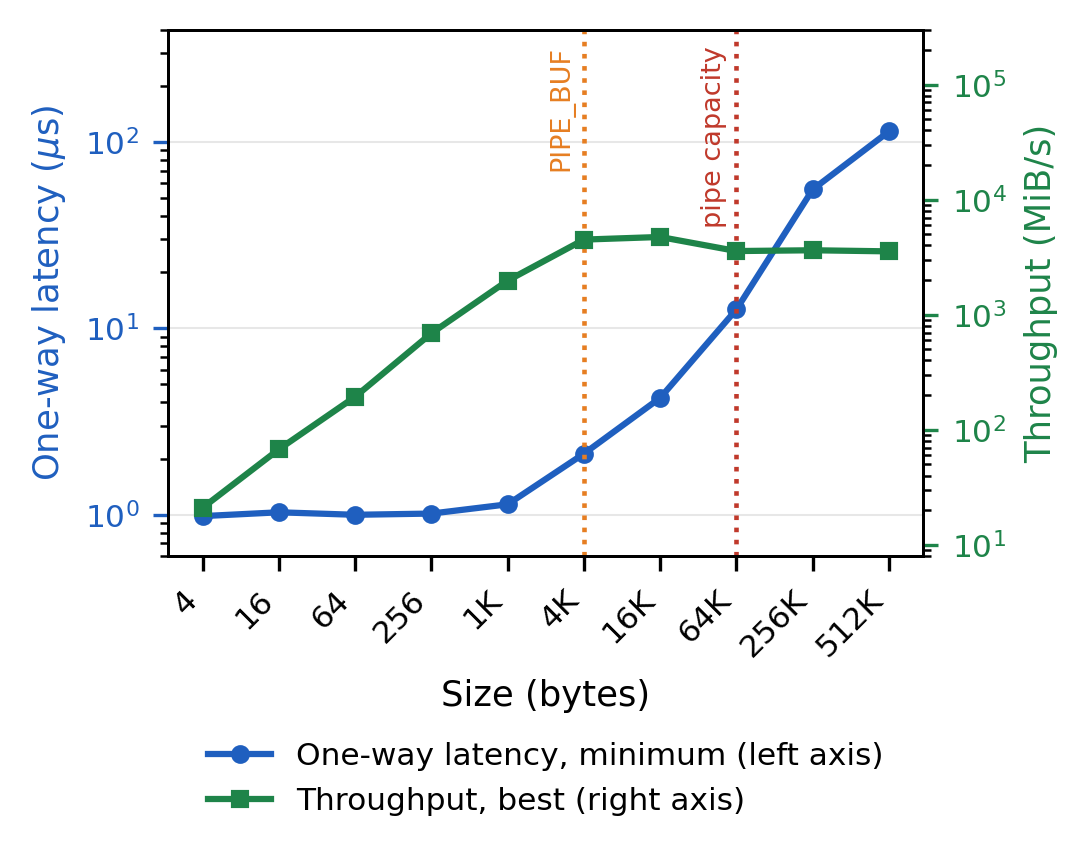
\includegraphics[width=1.0\linewidth]{latency_throughput.png}
    \caption{Pipe performance versus transfer size (parent on CPU~0, child on CPU~1, both at 4~GHz; five runs). Left axis (blue): minimum one-way latency, i.e.\ half the minimum round-trip time. Right axis (green): best throughput of a one-way stream. Both axes are logarithmic. Dotted lines mark \texttt{PIPE\_BUF} (4\,KB) and the pipe capacity (64\,KB).}
    \label{fig:lat-tp}
\end{figure}

Seen above are results for the pipe performance for throughput and one-way latency. What can be seen is that while the hypothesis holds partially for the 

TODO: Merge the two above.



\newpage
\newpage
\bibliographystyle{ACM-Reference-Format}
\bibliography{sample-base}

\end{document}
\endinput
%%
%% End of file `sigconf.tex'.

